%%%%%%%%%%%%%%%%%%%%%%%%%%%%%%%%%%%%%%%%%%%%%%%%%%%%%%
\documentclass[12pt,a4paper,oneside]{report}

%%%%%%%%%%%%%%%%%%%%% packages %%%%%%%%%%%%%%%%%%%%%
\usepackage[french]{babel} 
\usepackage[utf8]{inputenc}
\usepackage[T1]{fontenc}

\usepackage[table]{xcolor} %for colors

\usepackage{graphicx} % images, colors, etc
\usepackage[toc]{glossaries} % glossaries
\usepackage{pdfpages} % include pdf file in document
\usepackage{hyperref} % for references
\usepackage{float} % align figure
\usepackage{adjustbox}

\usepackage{tikz}% for diagram
\usetikzlibrary{shapes.geometric, arrows}

\usepackage{multirow} % mutliple row in tabular
\usepackage{hhline} % double hline in tabular

\usepackage{amsmath}%for math equation

\usepackage{wrapfig}% to wrap figure around text

%for subfigure
\usepackage{caption}
\usepackage{subcaption}

%for italic small caps
\usepackage{lmodern}% http://ctan.org/pkg/lmodern
\usepackage{slantsc}% http://ctan.org/pkg/slantsc

\usepackage[outputdir=out]{minted} % for code



%\usepackage{pstricks}
%\usepackage{auto-pst-pdf}

%\usepackage{enumitem}% control layout of the three basic list environments.



\usepackage{fancyhdr} % page style
\definecolor{ForestGreen}{RGB}{34,139,34}
\newcommand{\todo}[1]{\textcolor{ForestGreen}{\textbf{TODO: #1}}}
\newcommand*{\fullref}[1]{\hyperref[{#1}]{\autoref*{#1} \nameref*{#1}}}



%%%%%%%%%%%%%%%%%%%%% page style %%%%%%%%%%%%%%%%%%%%%
\pagestyle{fancy}

\setlength{\parindent}{1cm}
\newcommand{\textcalli}[1]{{\small{\textbf{$\negmedspace$\calligra #1}}}}

\renewcommand{\chaptermark}[1]{\markright{\thechapter\ #1}}
\renewcommand{\sectionmark}[1]{\markright{\thesection\ #1}}
\fancyhf{} % supprime les en-têtes et pieds prédéfinis
\fancyhead[R]{\thepage}% Left Even, Right Odd
%\fancyhead[R]{\textsl{\rightmark}}%moi
\fancyhead[L]{\textsl{\leftmark}} % Left Odd
%\fancyfoot[R]{\thepage} %moi
%\fancyhead[RE]{\textsl{\leftmark}} % Right Even
\renewcommand{\headrulewidth}{0pt}% filet en haut de page
\renewcommand{\footrulewidth}{0pt} % pas de filet en bas
\fancypagestyle{plain}{ % pages de tetes de chapitre
\fancyhead{} % supprime l’entete
\fancyhead[R]{\thepage}
\renewcommand{\headrulewidth}{0pt} % et le filet
}
%\makeglossaries
%\loadglsentries{glossaire.tex}

%%colors
\definecolor{dark}{HTML}{333333}
\definecolor{red}{HTML}{D1002E}
\definecolor{grey}{HTML}{888A8D}
\definecolor{white}{HTML}{FFFFFF}
\definecolor{blue}{HTML}{00ABD0}
\definecolor{green}{HTML}{00C048}

%%Flowcharts
%\tikzstyle{mydecision}=[diamond, draw=black, fill=grey, text=white!30, text centered, node distance=3cm]
\tikzstyle{endfail} = [rectangle, rounded corners, minimum width=3cm, minimum height=1cm,text centered, draw=black, fill=red]
\tikzstyle{endsuccess} = [rectangle, rounded corners, minimum width=3cm, minimum height=1cm,text centered, draw=black, fill=green]
\tikzstyle{process} = [rectangle, minimum width=3cm, minimum height=1cm, text centered, draw=black, fill=grey!30]
\tikzstyle{decision} = [diamond, minimum width=3cm, minimum height=1cm, text centered, draw=black, fill=dark!60]
\tikzstyle{arrow} = [thick,->,>=stealth]
 % load theme
%%%%%%%%%%%%%%%%%%%%%%%%%%%%%%%%%%%%%%%%%%%%%%%%%%%%%%
%%%%%%%%%%%%%%%%%%%%%%%%%%%%%%%%%%%%%%%%%%%%%%%%%%%%%%
\begin{document}

%%%%%%%%%%%%%%%%%%%%% title page %%%%%%%%%%%%%%%%%%%%%
\includepdf[pages=-]{page_garde/page_garde.pdf}

\pagenumbering{roman}

%%%%%%%%%%%%%%%%%%%%% thanks %%%%%%%%%%%%%%%%%%%%%
\chapter*{Remerciements}
\renewcommand{\leftmark}{REMERCIEMENTS}

    Nous remercions ...\\

\newpage

%%%%%%%%%%%%%%%%%%%%% table of contents %%%%%%%%%%%%%%%%%%%%%
\renewcommand{\leftmark}{TABLE DES MATI\`{E}RES}
\thispagestyle{fancy}
\tableofcontents

\newpage
%\listoffigures
\pagenumbering{arabic}
%%%%%%%%%%%%%%%%%%%%% intro %%%%%%%%%%%%%%%%%%%%%
%\renewcommand{\leftmark}{INTRODUCTION}
\chapter{Introduction}\label{chap:intro}

L'objectif de ce mémoire est de concevoir une architecture réseau permettant la communications avec des capteurs/actuateurs utilisés pour la surveillances de cultures.

Ce déploiment a les caractéristiques suivantes:
\begin{itemize}
    \item Les noeuds du réseau sont fortement contraints énergétiquement. Ils seront typiquement alimentés
    par une batterie éventuellement associée à des panneaux solaires et un régulateur de charge.
    \item Les caractéristiques des liens radio LoRa et IEEE 802.15.4 sont différentes et susceptibles
    de changer au cours du temps suite à par exemple, la croissance des feuilles des cultures surveillées.
    \item Le débit des transmissions n'a pas besoin d'être élevé.
\end{itemize}

Actuellement, il existe une multitude de protocoles radio ayant chacun leurs caractéristiques.
La figure \ref{fig:intro-linkStandard} illustre le débit et la portée de différents protocoles.
%todo choix du protocoles: pas haut datarate et lora longue portée et 802.15.4 courte portée.

\begin{figure}
    \centering
    \includegraphics[scale=0.3]{res/link-standard.png}
    \label{fig:intro-linkStandard}
    \caption{Débits de données et distances de transmission.}
\end{figure}

Le choix d'une architecture hybride réalisée avec LoRa et 802.15.4 semble donc le plus approprié
pour ce déploiment.

La solution proposée est développée sur la plateforme RE-Mote de Zolertia.
Cette plateforme possède les caractéristiques suivantes:
% ARM Cortex-M3 32-Mhz
% 32KB de RAM
% I2C, SPI, UART
% General Purpose Pin(GPIO)
% USB 2.0 12 Mbps
%Micro-SD
%Built-in LiPo battery Charger
%RF 2.4Ghz ISM 2.4GHz IEEE802.15.4, 250 Kbps avec modulation DSSS
%ISM 863-868,915-, 920-, 950MHz
%%%%%%%%%%%%%%%%%%%%% chapters %%%%%%%%%%%%%%%%%%%%%
\renewcommand{\leftmark}{ETAT DE L'ART}
\chapter{Etat de l'art}\label{chap:state}

\section{IEEE 802.15.4}\label{sec:etat_art-802.15.4}
\renewcommand{\rightmark}{IEEE 802.15.4}

  802.15.4 est un protocole définis par IEEE en 2003. Il est destiné aux
  communications à débit faibles réalsisées par des dispositifs ayant une
  alimentation en énergie limitée.
  Ce protocole, qui est un standart pour les réseaux PANs (Personak Area
  Networks) couvre la couche physique et MAC du modèle OSI.

\subsection{Types de noeuds}\label{subsec:etat_art-802.15.4.nodes}
  La norme 802.15.4 défini deux types de noeuds:
  \begin{itemize}[label=\textbullet]
    \item Les noeuds \textbf{FFD} (Full Function Device) peuvent être des corrdinateurs de PAN, de simple
          coordinateurs ou de simple noeuds.
    \item Les noeuds \textbf{RFD} (Reduced Function Device) utilisent une implémentation réduite du protocole
    et peuvent seulement opérer comme des simples noeuds.  
  \end{itemize}

\subsection{Topologies}\label{subsec:etat_art-802.15.4.topologies}
  Ces noeuds peuvent former des réseaux suivants plusieurs topologies: la topologie en étoile (Fig
  \ref{fig:etat_art-802.15.4.topology.star}) pour laquelle plusieurs RFD sont connectés à un FFD qui
  joue le rôle de coordinateur, la topologie peer-to-peer
  (Fig \ref{fig:etat_art-802.15.4.topology.p2p}) pour laquelle les FFD sont connectés les uns aux autres.
  \begin{figure}[H]
    \makebox[\textwidth][c]{
    \begin{minipage}{0.5\textwidth}
      \centering
      \includegraphics[scale=0.35]{images/802154_topologies_p2p.png}
      \caption{802.14.4 topologie peer-to-peer.}
      \label{fig:etat_art-802.15.4.topology.p2p}
    \end{minipage}
    \hspace{1cm}
    \begin{minipage}{0.5\textwidth}
      \centering
      \includegraphics[scale=0.35]{images/802154_topologies_star.png}
      \caption{802.15.4 topologie en étoile.}
      \label{fig:etat_art-802.15.4.topology.star}
    \end{minipage}}
  \end{figure}


\subsection{Beacon Enabled mode}\label{subsec:etat_art-802.15.4.be}
  Dans ce mode d'accès, le réseau est synchronisé par des messages de contrôles (beacons)
  et une structure appelée Superframe (Fig. \ref{fig:etat_art-802.15.4.superframe}).
  Cette Superframe est générée périodiquement par les coordinateurs.
  Elle est délimitée par des beacons qui sont émis à un intervalle \textit{beacon interval (BI)}
  qui est défini par le paramètre \textit{beacon order (BO)}
  $BI = 15.36 \cdot 2^{BO}\ avec\ 0 \leq BO \leq 14$.
  
  La superframe peut être divisée en deux périodes: la période active et la période inactive.
  La période active a une durée \textit{Superframe duration (SD)} qui est définie par 
  le paramètre \textit{Superframe order (SO)} $SD=15.36 \cdot 2^{SO}\ avec\ 0 \leq SO \leq BO \leq 14$.
  Elle est elle-même divisée en deux périodes:
  \textit{contention acces period (CAP)} et \textit{contention free period (CFP)}.
  %Pendant la CAP, l'accès au canal se fait par l'algorithme CSMA-CA (Carrier Sense Multiple Access with Collision Avoidance).
  %Pour la CFP, chaque noeud utilise un slot (Guaranteed Time Slots (GTS)) parmi les 7 disponibles.
  \begin{figure}[H]
    \centering
    \makebox[\textwidth]
    {
      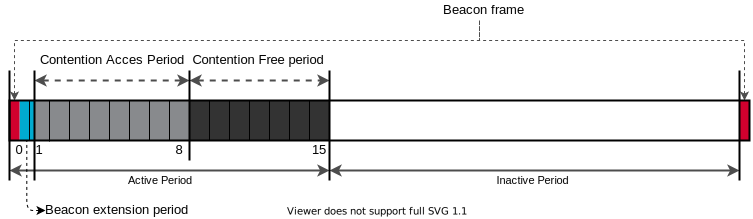
\includegraphics[scale=0.8]{images/superframe.png}
    }
    \caption{802.15.4 structure de la Superframe.}
    \label{fig:etat_art-802.15.4.superframe}
  \end{figure}

\subsubsection*{Accès au canal durant la contention acces period (CAP)}
  Durant cette période, l'accès au canal se fait par l'algotihme slotted CSMA-CA
  (Carrier Sense Multiple Access with Collision Avoidance). La figure~\ref{fig:etat_art-csmaca}
  illustre son fonctionnement.

  Les time slots de la CAP sont divisés en plus petits time slots appelés \textbf{backoff periods}.
  Un noeud du réseau maintient les variables suivantes:
  \begin{itemize}[label=\textbullet]
    \item $NB$ compte le nombre de backoff. Initialisée à 0
    \item $CW$ indique la taille de la fenêtre de congestion. Initialisée à 2
    \item $BE$ est l'exposant du backoff. Initialisée à macMinBE
  \end{itemize}

  Les variables macMinBE, macMaxBe et MCB (macCSMABackoffs) sont des constantes du protocole.
  Lorsque des paquets doivent être transmis, les variables sont d'abord initialisées.
  Ensuite, le noeud attend le prochain backoff et choisis aléatoirement un nombre entier
  $r r \in [0, 2^{BE}-1]$. Après avoir avoir attendu r backoff periods, le noeud vérifie
  si le canal est occupé en réalisant un CCA (Clear Channel Assessment).
  Si c'est le cas, $CW$ va être décrémenté et un nouveau CCA va être réalisé.
  Les paquets ne pourront être transmis qu'après trois CCA consécutifs indiquant un canal libre (i.e. $CW = 0$).
  Si le canal est occupé, $NB$ et $BE$ sont incrémentés et $CW$ est réinitialisé à 2.
  Enfin, si $NB$ n'exède pas \textit{macCSMABackoffs}, le noeud va reprendre à l'étape où un
  $r$ est choisis aléatoirement. Sinon, la communication ne sera pas établie et les paquets
  ne seront pas transférés.


\begin{figure}[H]
\begin{tikzpicture}[node distance=1.7cm]

  \node (start) [process] {\begin{tabular}{c} $NB = 0$; $CW = 2$ \\ BE = macMinBE \end{tabular}};
  \node (in1) [process, below of=start] {\begin{tabular}{c} wait until next backoff\\ period boundary\end{tabular}};
  \node (pro1) [process, below of=in1] {\begin{tabular}{c} Skip $r \in [0, 2^{BE}-1]$ \\ backoff periods \end{tabular}};
  \node (pro2) [process, below of=pro1] {Perform CCA};
  \node (dec1) [decision, below of=pro2, yshift=-0.8cm] {Channel idle?};

  \node (pro2a) [process, below of=dec1, yshift=-1cm] {\begin{tabular}{c} $NB = NB+1;CW = 2$ \\ $BE = min(BE+1, macMaxBE)$ \end{tabular}};
  \node (pro2b) [process, right of=pro2a, xshift=4cm] {$CW = CW-1$};
  \node (dec2) [decision, below of=pro2a, yshift=-1cm] {NB > MCB ?};
  \node (dec3) [decision, below of=pro2b, yshift=-1cm] {CW = 0\ ?};
  \node (fail) [endfail, below of=dec2, yshift=-1cm] {Failure};
  \node (success) [endsuccess, below of=dec3, yshift=-1cm] {Success};
  
  \draw [arrow] (start) -- (in1);
  \draw [arrow] (in1) -- (pro1);
  \draw [arrow] (pro1) -- (pro2);
  \draw [arrow] (pro2) -- (dec1);
  \draw [arrow] (dec1) -| node[anchor=south] {Yes} (pro2b);
  \draw [arrow] (dec1) -- node[anchor=east] {No} (pro2a);
  \draw [arrow] (pro2a) -- (dec2);
  \draw [arrow] (pro2b) -- (dec3);
  \draw [arrow] (dec2) -- node[anchor=east] {Yes} (fail);
  \draw [arrow] (dec2) -- node[anchor=south] {No} ++(-4,0) |- (pro1);
  \draw [arrow] (dec3) -- node[anchor=south] {No} ++(3,0) |- (pro2);
  \draw [arrow] (dec3) -- node[anchor=east] {Yes} (success);
  \end{tikzpicture}
  \caption{Schéma de l'algorithme slotted CSMA-CA.}
  \label{fig:etat_art-csmaca}
\end{figure}



\subsubsection{Accès au canal durant la contention free period} (CFP)
TODO

\subsection{Non-Beacon Enabled mode}\label{subsec:etat_art-802.15.4.nbe}

\subsection{Adressage}\label{subsec:etat_art-802.15.4.adress}

\subsection{Mécanisme d'Ack optionnel}\label{subsec:etat_art-802.15.4.ack}

\newpage
\section{RPL}\label{sec:state-rpl}
\renewcommand{\rightmark}{RPL}
%TODO tour des protocoles de routages ??

Routing Protocol for Low-Power and Lossy Networks (RPL) est un protocole de routage IPv6 destiné aux réseaux dont les noeuds sont contraints en énergie et dont les liens entre ces noeuds sont soumis à des pertes importantes de paquets (Low-power and Lossy Networks (LLNs)).
Ce protocole à vecteur de distance est un protocole proactif, c'est à dire que les routes sont établies avant qu'elles ne soient nécessaires.

RPL sépare le traitement et la transmission des paquets de l'optimisation de l'objectif de routage. Cela permet de l'adapter à un large éventail d'applications des LLNs.

\subsection*{Topologie}
%TODO exemple de topologie + collect application noeuds-> racine
La topologie utilisée par RPL et le DODAG (Destination Oriented Dag). Un DODAG est un graphe dirigé acyclique (DAG) ayant une seule racine.
\begin{figure}[H]
    \centering
    \includegraphics[scale=0.45]{res/dodag.drawio.png}
    \caption{DODAG.}
    \label{fig:state-dodag}
\end{figure}


\subsection*{Fonctions objectif}
%TODO expliquer brievement MRHOF et 0F0 (celles implémentées dans contiki)
Une fonction objectif (OF) défini comment plusieurs métriques sont utilisées pour calculer le rang d'un noeud. Le rang d'un noeud détermine sa position dans le DODAG par rapport aux autres noeuds.
Le rang augmente stictement dans le sens descendant et diminue strictement dans le sens montant. Ainsi, $rang(n)>rang(parent(n))$. La figure~\ref{fig:state-dodag} illustre un DODAG avec des valeurs de rang fictives attribuées aux noeuds. Sur cet exemple, la racine du DODAG a comme range, la valeur par défaut \textsc{root\_rank} définie dans le RFC.

Cette section décris brièvement deux fonctions objectif implémentées dans Contiki: OF0 et MRHOF.
\begin{itemize}
    \item \subsubsection*{OF0}%rfc6552
            Objective Function Zero est une fonction dont l'objectif est de choisir un parent qui permettra à un noeud d'avoir la racine du DODAG le plus proche possible. Le rang d'un noeud $R(N)$ est calculé comme suit:
            \begin{equation}
                ranck\_increase = (Rf * Sp + Sr) * MinHopRankIncrease
                \newline
                R(N) = R(P) + ranck\_increase
            \end{equation}
    \item \subsubsection*{MRHOF}
            Minimum Rank with Hysteresis Objective Function
\end{itemize}




\subsection*{Types de messages}
%TODO décrire le format des différents messages

\subsection*{Construction du réseau}
%TODO décrire les étapes de construction d'un réseau

\subsection*{Modes de fonctionnements}
%TODO parler des différents modes de fonctionnement: Storing mode/non-storing mode

\subsection*{Discussion}
%TODO RPL good parce que fait pour LLN (intro article eval RPL) et implémenté dans Contiki mais améliorations pour l'exterieur et grands réseaux (conclusion article eval RPL)
%%bib:
%@INPROCEEDINGS{5464820,
%  author={Tripathi, J. and de Oliveira, J. C. and Vasseur, J. P.},
%  booktitle={2010 44th Annual Conference on Information Sciences and Systems (CISS)}, 
%  title={A performance evaluation study of RPL: Routing Protocol for Low power and Lossy Networks}, 
%  year={2010},
%  volume={},
%  number={},
%  pages={1-6},
%  doi={10.1109/CISS.2010.5464820}}
\section{RTOS}

Un RTOS (Real Time Operating System) est un sytème d'exploitation temps réels principalement destiné aux systèmes embarqués.

Etant donné que ce projet utilise le protocole 802.15.4 ainsi que TSCH, le RTOS choisis doit les prendre en charge ainsi qu'un ou plusieurs algorithme d'ordonnancement de TSCH.

Il est également préférable, que le RTOS choisis, supporte déjà la plateforme utilisée. Une implémentation de la LoRa n'est pas nécessaire car les communications Lora sont réalisées via le RN2483 qui est controlé par UART.

Pour effectuer ce choix, les RTOS suivants ont été comparés: Contiki OS, FreeRTOS, RIOT OS et Zephyr.

\subsection*{Contiki OS}
    Le développement publique de Contiki a débuté en octobre 2012\footnote{Date de création du repository Github.}. Dans un premier repository: \textbf{contiki}~\cite{contiki-repo:old}. Un nouveau développement a démarré en mai 2017 sous le nom de \textbf{contiki-ng}~\cite{contiki-repo:ng}. C'est donc ce dernier qui est utilisé pour la comparaison est qui est dénommé par la suite "Contiki".

    Cet OS open-source et multi-plateforme implémente toute une série de protocoles de communications basse énergie tels que IEEE 802.15.4, 6TiSCH, IPv6/6LoWPAN et RPL. En plus de 6TiSCH, un ordonnanceur TSCH, Orchestra, est implémenté.

    L'implémentation des processus est basée sur la librairie Protothreads~\cite{paper:protothreads}
    qui abstrait la gestion de la programmation évènementiel par des protothread dont l'utilsations est similaire aux threads. L'ordonnenceur de cette libraire est cooperatif, c'est à dire qu'il ne va jamais forcer un changement de contexte d'un processus à un autre. Le changement de contexte ne s'effectue que quand un processus rend volontairement le contrôle à l'ordonnanceur.
    
    Contiki est également compatible avec le Zolertia RE-Mote. Il est accompagné de Cooja, un simulateur réseau qui permet de simuler les communications entre plusieurs noeuds utilisant Contiki.

\subsection*{FreeRTOS}
    D'après le site officiel de FreeRTOS~\cite{freertos}, ce RTOS est développé depuis 15 ans.
    TODO compatible avec zolertia ?
    \todo{fifi}

\subsection*{RIOT OS}
    Le développement publique de RIOT a débuté en décembre 2012\footnotemark[1].
    
    D'après le site officiel, cet OS supporte 229 carte de développement et 64 CPU dont le Zolertia RE-Mote. 

    La pile réseau de RIOT comporte les protocoles notemment 6LoWPAN, IPv6, RPL, LoRaWan, 802.15.4.
    TODO openwsn

\subsection*{Zephyr}
    TODO pas supporté 
    tiny os plus de commit depuis 1 an. stack réseau ? supporté ?

Le table~\ref{tb:state-rtos-choice} résume la comparaison de ces RTOS.

Le RTOS choisi est Contiki OS. Il a été choisi pour sa maturié, la prise en charge du Zolertia RE-Mote et sa pile réseau complète.


%https://github.com/Lora-net/LoRaMac-node/blob/ba17382bd5109513937afad07f068a781a503ef6/src/radio/radio.h
\begin{table}[H]
    \begin{adjustbox}{width=\textwidth}
        \begin{tabular}{c||c|c|c|c|c|c|c}
            RTOS & 802.15.4 & ord. TSCH & LoRa & IPv6 & routage IP & comp. \\ \hline

            \textbf{Contiki OS} & $\surd$  & 6Tisch, Orchestra & Projet KRATOS & $\surd$ & RPL        & $\surd$ \\ \hline

            FreeRTOS            & $\times$ & $\times$          & $\surd$       & $\surd$ & $\times$   &    $\times$     \\ \hline

            RIOT OS             & $\surd$  & $\times$          & $\surd$       & $\surd$ & RPL        &    $\surd$     \\ \hline

            Zephyr              & $\surd$  & $\times$          & $\surd$       & $\surd$ & Thread     &    $\times$     \\
        \end{tabular}
    \end{adjustbox}
    \caption{Comparatif de différents RTOS.}
    \label{tb:state-rtos-choice}
\end{table}
TODO supprimer colonne LoRa mais citer kratos ? 

\renewcommand{\leftmark}{ARCHITECTURE}
\chapter{Architecture}\label{chap:archi}

\section{Topologie}\label{sec:archi-topologie}
\renewcommand{\rightmark}{Topologie}

Cette section décrit et motive la topologie et les types de noeuds du réseau hybride IEEE 802.15.4-LoRa de capteurs. Cette topologie a été choisie pour correspondre au mieux au cas d'utilisation décrit dans l'introduction.\todo{REF INTRO}

\subsection*{Types de noeuds}
    Le protocole élaboré pour ce réseau hybride défini 3 types de noeuds:
    \begin{itemize}
        \item[-] La \textbf{racine LoRa} est la passerelle entre le réseau et un réseau IP externe. Elle possède donc une interface LoRa et par exemple une interface Wi-Fi.
        \item[-] La \textbf{racine RPL}, comme son l'indique, est la racine d'un réseau RPL. Elle possède également une interface LoRa pour communiquer avec la racine LoRa.
        \item[-] Les \textbf{noeuds RPL} sont des noeuds du réseau RPL.
    \end{itemize}

\subsection*{Topologie}
Comme l'illustre la figure~\ref{fig:archi-topologie} la topologie choisie est une topologie mixte.

On a d'abord un ensemble de réseaux RPL possèdant chacun un préfixe IP attribué par la racine LoRa (par exemple $0x02$ ou $0x04$ sur la figure~\ref{fig:archi-topologie}), dans lesquels les communications sont réalisées par des liens IEEE 802.15.4.
De part l'utilisation de RPL, chaque réseaux forme un DODAG.

Ensuite, chaque réseau RPL est connecté à la racine LoRa via sa racine. Les liens entre les racines RPL et la racine LoRa forment une topologie en étoile.

Ce choix de topologie offre plusieurs avantages: Le fait d'avoir un ensemble de réseaux RPL implique qu'il n'y a pas qu'une seule racine RPL et donc pas qu'un seul point de défaillance; L'administration du réseau est également simplifiée. En effet, un réseau RPL pourraît, par exemple, correspondre à une parcelle de terrain. 

L'inconvéninent de cette topologie est que la racine LoRa constitue un seul point de défaillance. Une solution plus robuste qui a été envisagée, est un réseau maillé pour les communications LoRa. Cependant, une telle architecture est difficile à mettre en oeuvre car le protocole MAC a établir pour les liens LoRa est plus complexe et nécessite un protocole de routage.

\begin{figure}[H]
    \centering
    \includegraphics[scale=0.7]{res/pictures/loramac-topologie.drawio.png}
    \caption{Topologie du réseau hybride.}
    \label{fig:archi-topologie}
\end{figure}

Ainsi, l'objectif de cette topologie est de transmettre les paquets IP à destination de la racine LoRa.
\section{Format d'adresse}\label{sec:archi-adresses}
\renewcommand{\rightmark}{Format d'adresse}

Cette section décrit les possibilités envisagées pour le choix du format des adresses utilisées pour les communications LoRa et motive le choix d'un format. Dans chaque hypothèse, un réseau RPL possède un préfixe de sous-réseau qui lui est propre.

\subsection*{Adresse IPv6}
    La première solution envisagée est d'utiliser les adresses IPv6 des noeuds.
    Une racine RPL peut ainsi vérifier si un paquet est destiné à son réseau et la racine LoRa à elle même,
    via le préfixe de sous réseau de l'adresse de destintation.
    Cette solution est la plus simple à mettre en oeuvre car elle ne nécéssite pas de table de routage ou de processus de conversion d'adresse. Cette approche a néanmoins le désavantage que les adresses IP de 128 bits sont transportées sur un lien LoRa ce qui représente un temps de transmission important.
    
    Néanmoins la taille des adresses IP est de 128 bits.

\subsection*{Préfixe et \textit{node-id}}
    Une seconde approche est d'utiliser un préfixe et le \textit{node-id}. Ce dernier est un identifiant de noeud sur 16 bits utilisé dans Contiki. Son calcul, basé sur les deux derniers octets de l'adresse MAC du noeud (\textit{link-layer address}) est le suivant:
    \[
        node\_id = link\_addr[s-1] + (link\_addr[size -2] << 8)
    \]
    où $s$ est la taille de la \textit{link-layer address}.\\

    Le format d'adresse utilisé serait alors un préfixe sur 8 bits et le \textit{node-id} sur 16 bits ce qui fait un total de 24 bits.

    L'avantage de cette solution est que la taille des adresses est réduite d'un facteur de 18,75\%. Néanmoins, un processus de conversion est nécessaire ainsi qu'une table de conversion d'un \textit{node-id} vers une adresse MAC pour chaque noeud RPL. En effet, le calcul du \textit{node-id} ne permet pas de reconstituer l'adresse MAC de 64 bits à partir de celui-ci.
    Un autre inconvénient est que l'utilisation du préfixe de 8 bits limite le nombre de réseaux RPL à 256, ce qui reste néanmoins acceptable.
    % === infos ===
    % Dans contiki, la link layer address est "remplie" dans arch/zoul/platform.c par
    % `ieee_addr_cpy_to(linkaddr_node_addr.u8, LINKADDR_SIZE);` qui est définie dans
    % arch/cpu/cc2538/iee-addr.c qui va lire l'adresse dans la mémoire flash du cc2538
    % sauf si IEEE_ADDR_CONF_HARDCODED est définie. Dans ce cas c'est une adresse harcodée
    % qui est utilisée
    %

\subsection*{Préfixe et adresse MAC}
    Pour résoudre le problème de la conversion \textit{node-id}$\leftrightarrow	$ adresse MAC, cette solution consiste à remplacer le \textit{node-id} par l'adresse MAC d'un noeud.

    Cette solution permet une conversion d'adresse simple et la taille des adresses est de 72 bits (64 bits de l'adresse MAC et 8 bits du préfixe).

\subsection*{Solution retenue}
    La solution retenue est l'utilisation du préfixe de 8 bits et du \textit{node-id} car c'est la solution qui offre les adresses les plus courtes. Pour éviter l'utilisation d'une table de conversion \textit{node-id}$\leftrightarrow$ adresse MAC, une meilleure solution que d'utiliser les adresses MAC des noeuds et de modifier les 6 premiers octets de cette dernière. Cela permet de reconstituer une adresse IPv6 simplement, mais cela réduit le nombre d'adresses possible
    Malgré tout, le nombre d'adresse possible reste largement suffisant pour ce projet.

    L'adresse de la racine LoRa est une adresse configurée administrativement.

    %todo schéma conversion, adresse de la racine 
\section{Trames LoRaMAC}\label{sec:archi-loramac-frame}
\renewcommand{\rightmark}{Trames LoRaMac}

    Le protocole MAC mis en place pour les communications LoRa utilise un seul format de trames illustré à la figure~\ref{fig:archi-frame}.
    \begin{figure}[H]
        \centering
        \includegraphics[scale=0.5]{res/pictures/loramac-frame.drawio.png}
        \caption{Format de trame LoRaMAC.}
        \label{fig:archi-frame}
    \end{figure}
    Les trames LoRaMAC sont composées des champs suivants:
    \begin{itemize}
        \item \textbf{dest\_addr}: l'adresse de destination (24 bits)
        \item \textbf{src\_addr}: l'adresse source (24 bits)
        \item \textbf{K}: un flag  qui indique si la trame nécessite un acquittement (1 bit)
        \item \textbf{next}: un flag qui indique si une autre trame suit (1 bit)
        \item \textbf{reserved}: 2 bits réservés pour évolution future
        \item \textbf{command}: la commande MAC (4 bits).\\
        Les 5 commandes disponibles ainsi que leurs valeurs sont reprises dans la table~\ref{tb:archi-loramac-command}. Il est possible d'ajouter 10 commandes supplémentaires pour des usages futurs.
        \item \textbf{SN}: le numéro de séquence de la trame (8 bits)
        \item \textbf{Payload}: la payload ayant une taille maximale de 247 octets. Cette limitation provient de la radio LoRa utilisée, le RN2483, qui limite les transmissions à 255 octets, valeur de laquelle est soustrait les 8 octets des champs précédents.
        \begin{table}[H]
            \centering
            \makebox[\textwidth]{%
            \begin{tabular}{|c|c|c|c|}
                \hline
                Valeur & Commande & description & payload\\ \hline
                0 & JOIN & requête pour rejoindre le réseau & $\times$ \\ \hline
                1 & JOIN\_RESPONSE & réponse à la commande JOIN & préfixe du sous réseau\\ \hline
                2 & DATA & transport de données & données\\ \hline
                3 & ACK & acquittement & $\times$\\ \hline
                4 & QUERY & demande de trafic descendant & $\times$\\ \hline
            \end{tabular}
            }
            \caption{Description des commandes LoRaMAC.}
            \label{tb:archi-loramac-command}
        \end{table}
    \end{itemize}

\section{LoRaMAC}\label{sec:archi-loramac:proto}
\renewcommand{\rightmark}{LoRaMac}

    Cette section décris le protocole MAC mis en place pour les communications LoRa. Ce protocole est donc utilisé pour les communications entre la racine LoRa et les racines RPL. Ces dernières étant contraintes en énergie, leur radio LoRa n'est pas tout le temps allumée. Le protocole prend donc en compte cette contrainte.

\subsection{Etats d'une Racine RPL}
    Les racines RPL, utilisent 3 états. A l'initiation du réseau, une racine RPL se trouve dans l'état \textit{alone}. Elle demande ensuite son préfixe à la racine LoRa, et une fois celui-ci reçu, la racine RPL se trouve dans l'état \textit{ready}. Quand une racine RPL envoie une trame qui nécéssite un acquittement, tant que celui-ci n'est pas reçu elle se trouvera dans l'état \textit{wait\_response}. Une fois l'acquittement reçu, elle retournera dans l'état \textit{ready}.
    Les trames qui doivent être envoyées le seront en fonction de l'état dans lequel se trouve une racine RPL. Dans l'état \textit{ready}, les trames peuvent être envoyées mais ce n'est pas le cas dans les états \textit{alone} et \textit{wait\_response}. En effet dans le premier la racine RPL ne peut pas envoyer de données car elle n'a pas encore rejoint le réseau et dans le second, elle attend un acquittement.

\subsection{Construction du réseau}
    A l'initialisation du réseau, une racine RPL, doit envoyer une trame avec la commande MAC JOIN. Une fois reçue par la racine LoRa, celle-ci va répondre avec une trame JOIN\_RESPONSE qui fait office d'acquittement de la trame JOIN et dont la payload est le préfixe IP que la racine RPL doit diffuser dans son réseau.

    Si le trame JOIN ou la trame JOIN\_RESPONSE ne sont pas reçues, la racine 

\subsection{Communications montantes}

\subsection{Communications Descendantes}

\subsection{Gestion des numéros de séquence}

\subsection{Evitement de collision}

\renewcommand{\leftmark}{MISE EN OEUVRE}
\chapter{Mise en oeuvre}\label{chap:work}
    Ce chapitre décrit la mise en oeuvre de l'architecture définie dans le
    chapitre~\ref{chap:archi}.
    % on fait d'abord python puis c

    Deux implémentations sont réalisées. Celle de la racine LoRa en Python 3.8.10 et celle de la racine RPL avec la version\\ \texttt{Contiki-NG-develop/v4.7-18-ga3f6b04c5} de Contiki.

    Chaque implémentation est divisée en trois parties analogues aux couches physique, liaison et réseau du modèle OSI. La chouche physique est un driver permettant d'abstraire les communications UART avec le RN2483, rendant sont utilisation plus facile. La couche liaison implémente le protocole LoRaMAC, et la couche réseau sert d'interface permettant d'envoyer ou de recevoir des paquets IPv6.
\section{Racine LoRa}\label{sec:work-lora-root}
\renewcommand{\rightmark}{Trames LoRaMac}

    Cette section décrit l'implémentation de l'architecture pour la racine LoRa.
    L'implémentation se présente sous forme d'un package python qui donne accès à une variable NETWORK\_STACK qui fait référence à un objet NetworkStack qui permet d'accèder aux trois différentes couches, l'adresse LoRaMAC du noeud, son adresse IPv6 issue de la conversion de son adresse LoRaMAC ainsi que trois fonctions: init, send et register\_listener qui sont des fonctions de l'interface IP et permettent respectivement d'initialiser la pile réseau, d'envoyer des paquets IPv6 et d'enregister une fonction callback qui sera appelée lorsqu'un paquet IPv6 reçu est disponible. L'usage et l'implémentation de ses fonctions sont détaillées dans la description de la \nameref{subsec:work-loraroot:iplayer}.

\subsection*{Couche physique}
    La couche physique définit le format des adresses et trames LoRaMAC, ainsique que le driver 
    permettant de simplifier l'utilisation du RN2483 par l'abstraction des communications UART.

    La classe LoraAddr qui définit les adresses LoRaMAC, possède deux attributs entier qui sont le préfixe de l'adresse et le node-id. Cette classe possède également une fonction toHex() qui permet de sérialiser une adresse. C'est à dire de la convertir en une chaine de caractères hexadecimal qui est le format de donnée demandé par le RN2483.

    La classe LoraFrame qui définit une trame LoRaMAC possède comme attributs tous les champs d'une trame LoRaMAC. C'est à dire, les adresses source et destination, la commande MAC dont le type choisi est une énumération, la payload, le numéro de séquence et deux booléens pour les flags k et has\_next. COmme la classe LoraAddr, elle possède une fonction toHex mais également une fonction build(data: str) qui retourne une instance d'une LoraFrame construite sur base d'une chaine de caractères hexadécimal.

    Ces deux classes utilisent l'annotation @dataclass qui génère des fonctions spéciales comme \_\_init\_\_() et \_\_repr\_\_() automatiquement à partir d'une suite d'attributs en utilisant les annotations de type. Pour la classe LoraAddr, le paramètre de l'annotation frozen est mis à True pour rendre cette classe immuable.

    Le driver du RN2483 est implémenté par la classe LoraPhy qui ne possède que des attributs destinés à un usage interne. Son constructeur nécéssite néanmoins deux paramètres, le baudrate et le port de la connection série.

    La première fonction qui doit être appellée avant tout interraction avec le RN2483 est la fonction init(). Cette fonction ouvre la connexion série en instanciant un objet Serial de la librairie python pyserial version 3.4, démarre deux Threads utilisés pour les communications entrantes et sortantes et envoi les deux premières trames UART permettant de désactiver le protocole MAC, LoRaWAN, présent sur le RN2483 et de définir la fréquence radio utilisée.

    L'envoi des deux premières trames UART se fait via une fonction interne \_send\_phy(data: UartFrame). Cette fonction ajoute la trame UART passée en paramètre dans un buffer d'envoi s'il n'est pas complètement rempli. 
    Une trame UART est définie par la classe UartFrame, également une dataclass, qui possède trois attributs:
    \begin{itemize}
        \item expected\_response est de liste de réponses attendues en retour de l'envoi de cette trame. Les réponses possibles du RN2483 sont repris dans une énumération. 
        \item cmd est la command UART qui est également une énumération. Une commande UART est par exemple, "mac pause" pour désactiver LoRaWAN ou encore "radio tx" pour transmettre des données.
        \item data qui est une chain de caractères représentant les données suivant la commande UART. Cette chaîne de craractère peut être vide pour certaines commandes comme "mac pause".
        L'assemblage de cmd et data donne une trame UART. Par exemple pour transmettre les données "AB16FD", la command UART est radio tx AB16FD"
    \end{itemize}

    Une fois qu'une trame a été ajoutée au buffer d'envoi, le Thread \_uart\_tx va se charger de 
    son envoi. Le buffer d'envoi (comme le buffer de réception) est une Queue FIFO de la librairie 
    python queue.
    
    Pour récupérer une trame, il faut que une réponse correcte de la trame précédente ai été reçue ou que la trame a envoyée soit la première.
    Pour déterminer si une trame peut être envoyée le Thread vérifie que la connection série existe et que l'attribut du driver, \_can\_send, est vrai. Dans le cas contraire, le Thread est bloqué par une variable conditionelle \_can\_send\_cond également attribu du driver.
    La trame à envoyée est récupérée via une fonction get dont le paramètre block est 
    mis à True, ce qui bloque le Thread quand aucune donnée n'est disponible dans le buffer et évite donc de consommer des ressources. Une fois la trame envoyée, un attribut du driver, \_can\_send est mis à False.

    Le Thread \_uart\_rx lis les données de la connexion série via la fonction readline() de la classe Serial. Cette méthode bloque le Thread jusqu'au moment où une ligne peut être lue sur la connexion série. Une fois la ligne reçue, celle 







\subsection*{Couche MAC}

\subsection*{Couche IP}\label{subsec:work-loraroot:iplayer}
\section{Racine RPL}\label{sec:work-rpl-root}
\renewcommand{\rightmark}{Racine RPL}

    Dans la topologie choisie à la section \ref{sec:archi-topologie}, une racine RPL est la plateforme de développement Zolertia RE-Mote Rev.B à laquelle la carte d'interface du RN2483 a été raccordée par des câbles de prototypage. La figure~\ref{fig:work-montage} illustre le raccordement entre le RN2483 et le Zolertia.
    
    \begin{figure}[H]
        \centering
        \includegraphics[scale=0.35]{res/pictures/montage.png}
        \caption{Schéma du raccordement du RN2483 au Re-Mote.}
        \label{fig:work-montage}
    \end{figure}

    Comme l'indique la table~\ref{table:work-pin-description} de description des pins, les pins PC2 et PC3 utilisés pour la connexion ne sont pas ceux défini pour l'usage d'une connexion UART. Ces pins sont choisis pour la connexion UART car ils sont accessibles à l'exterieur du boitier de la plateforme par un connecteur.
    
    Pour que la connexion UART avec le RN2483 soit possible via les pins choisis, des modifications 
    dans Contiki du fichier de configuration de la plateforme sont nécéssaires.
    Ainsi, les valeurs des macros suivantes ont été modifiées dans le fichier \texttt{arch/cpu/cc2538/cc2538-conf.h}:
    \begin{itemize}
        \item \texttt{UART1\_CONF\_BAUD\_RATE} est définie à $57600$ qui est le baudrate par défaut du RN2483
        \item \texttt{UART1\_RX\_PIN} est définie à $2$
        \item \texttt{UART1\_TX\_PIN} est définie à $3$
    \end{itemize}

    Comme pour l'implémentation de la racine LoRa, celle de la racine RPL est réalisée en 3 couches.
    qui sont intégrées dans Contiki comme un service. C'est à dire que le code des 3 couches se trouve dans le répertoire suivant: \texttt{os/services/loramac}.
    
    \begin{table}[H]
        \centering
        \makebox[\textwidth]{%
        \begin{tabular}{|l|l|l|l|}
        \hline
        \rowcolor[HTML]{C0C0C0} 
        Pin & Default name       & MC  & Description                                                                            \\ \hline
        4   & UART0.RX           & PA0 & Connected to the CP2104 USB-to-serial converter                                        \\ \hline
        5   & UART0.TX           & PA1 & Connected to the CP2104 USB-to-serial converter                                        \\ \hline
        6   & GPD0/I2C.Interrupt & PD0 & Generic pin, may be used as auxiliary pin for I2C/SPI                                  \\ \hline
        7   & I2C.SDA            & PC2 & \multicolumn{1}{p{10cm}|}{GPIO 20 mA output capability, pull-up. Shared with the RTCC and on-board low-power PIC} \\ \hline
        8   & I2C.SCL            & PC3 &  \multicolumn{1}{p{10cm}|}{GPIO 20 mA output capability, pull-up. Shared with the RTCC and on-board low-power PIC} \\ \hline
        9   & DGND               & N/A & Digital Ground                                                                         \\ \hline
        10  & D+3.3              & N/A & 3.3VDC output pin                                                                      \\ \hline
        11  & CC1200.GPIO0       & PB4 &  \multicolumn{1}{p{10cm}|}{CC1200 GPIO0 pin. If RF switch disables sub-GHz is available for other purposes}        \\ \hline
        12  & CC1200.GPIO2       & PB0 &  \multicolumn{1}{p{10cm}|}{CC1200 GPIO2 pin. If RF switch disables sub-GHz is available for other purposes}        \\ \hline
        13  & UART1.RX           & PC1 &  \multicolumn{1}{p{10cm}|}{GPIO 20 mA output capability, no pull-up or pull-down.}                                 \\ \hline
        14  & UART1.TX           & PC0 &  \multicolumn{1}{p{10cm}|}{GPIO 20 mA output capability, no pull-up or pull-down.  }                               \\ \hline
        \end{tabular}%
        }
        \caption{Extrait de la table de descrition des pins~\cite{zolertia-remote:datasheet}.}
        \label{table:work-pin-description}
        \end{table}
\newpage
\subsection*{Couche physique}
    Comme pour la racine LoRa, la couche physique définit les trame et les adresses LoRaMAC et sert 
    de driver pour le RN2483. La réception et l'envoi de trames UART est réalisée par deux 
    processus.

    Le processus de récéption permet d'éviter que le reste du code soit interrompu par une trame 
    UART entrante. Le code suivant illustre la déclaration de processus dans contiki.  

    \begin{minted}[linenos]{c}
PROCESS_THREAD(ph_rx, ev, data){
    PROCESS_BEGIN();
    /* UART configuration */
    uart_init(UART);
    uart_set_input(UART, &uart_rx);
    PROCESS_END();
}
    \end{minted}
    Tout ce qui se trouve entre les instructions des lignes 2 et 6 dépend du processus. Ainsi, la 
    fonction, \texttt{uart\_rx} qui traite les trames UART entrantes dépend bien de ce processus.
    Le rôle de cette fonction est d'accumuler tous les caractères d'une trame UART pour ensuite 
    appeler une fonction qui traîte cette trame. Elle supprime également les caractères ayant comme 
    valeur entière 254, 248, 192 et 240. Ces caractèrent apparaissent lors de certaines réponses 
    UART et perturbe la reconstruction de la trame. La cause de l'apparition de ces caractères 
    n'est pas identifiée.

    Une fois la trame UART assemblée, une fonction suivante vérifie si cette réponse est une 
    réponse attendue pour la trame précédemment envoyée. Si c'est le cas, elle envoie un évènement 
    qu'attend le processus d'envoi pour envoyer la prochaine trame UART. Si la trame UART reçue 
    contient la commande \textit{"radio\_rx"}, la fonction construit une trame LoRaMAC et l'envoie 
    à la couche supérieure.

    Le processus d'envoi apour rôle d'envoyer toutes les trames UART présentes dans le buffer 
    d'envoi. Il peut être bloqué si le buffer d'envoi est vide ou s'il attend une réponse à la 
    dernière trame envoyée. Si le buffer d'envoi est vide, le processus sera débloqué par la 
    réception de l'évènement \texttt{new\_tx\_frame\_event}, et s'il attend une réponse, il sera 
    débloqué par la réception de l'évènement \texttt{can\_send\_event}.

    Dans Contiki, les évènements sont créés et envoyé de la manière suivante:
    \begin{minted}[linenos]{c}
        process_event_t new_tx_frame_event = process_alloc_event();
        process_post(&ph_tx, new_tx_frame_event, NULL);
    \end{minted}
    
    Le type type \texttt{process\_event\_t} est en réalité un \texttt{unsigned char} qui est incrémenté à chaque appel de \texttt{process\_alloc\_event()}.

    Les fonctions publiques de la couche physique sont les suivantes:
    \begin{itemize}
        \item \textbf{\texttt{void phy\_init()}}\\
            Initialise la couche physique. C'est à dire, alloue les évènements, démarre les 
            processus et envoie les trames UART permettant de mettre en pause LoRaWAN et de définir 
            les paramètres de la radio.
        \item \textbf{\texttt{void phy\_register\_listener(int (* listener)(lora\_frame\_t frame)})}\\
            Enregistre la fonction callback qui sera appelée lorsqu'une trame LoRaMAC est reçue.
        \item \textbf{\texttt{int phy\_tx(lora\_frame\_t frame)}}\\
            Envoie une trame LoRaMAC.
        \item \textbf{\texttt{int phy\_timeout(int timeout)}}\\
            Définis le temps d'expiration du watchdog timer.
        \item \textbf{\texttt{int phy\_sleep(int duration)}}\\
            Met le RN2483 en mode sommeil.
        \item \textbf{\texttt{int phy\_rx()}}\\
            Met le RN2483 en mode réception.
    \end{itemize}

    Toues ces fonctions créent une trame UART qu'elle ajoute au buffer d'envoi.

\subsection*{Couche MAC}
    La couche MAC définit 3 états: \textsc{alone}, \textsc{ready} et \textsc{wait\_response}.
    Ces états correspondent à ceux défini dans la section~\ref{sec:archi-loramac:proto}, mis à part l'état \textsc{sleep} qui n'a pas 
    besoin d'être défini explicitement, car dans cet état, le noeud attend, et donc rien d'autre ne peut se 
    passer. En effet, comme le noeud ne peut basculer dans cet état que si le transmission d'une 
    trame JOIN a échouée (i.e. après trois retransmissions), et qu'aucune trame LoRaMAC ne peut être reçue il impossible qu'il bascule dans cet état.
    De plus, aucune trame ne peut être envoyée, car tant que le noeud n'a pas rejoint le réseau LoRaMAC, 
    la radio 802.15.4 et le protocole de routage RPL ne sont pas actifs.
    Le premier état est l'état initiale, le second est utilisé quand la racine RPL est prête à 
    envoyer une trame et le dernier est utilisé quand elle attend une réponse à une trame envoyée.

    Cette implémentation utilise un processus qui envoi les trames disponibles dans un buffer. 
    Ce processus peut être bloqué si le buffer est vide ou si l'état est différent de \textsc{ready}. Il peut être débloqué respectivement par les évènements
    \texttt{new\_tx\_frame\_event} et \texttt{state\_change\_event}. Ce processus démarre également un timer, \texttt{retransmit\_timer} lorsqu'une trame attend une réponse en retour. C'est à dire, lorsqu'il envoie une trame QUERY ou une trame avec le flag k à \textit{true}.
    
    Comme pour l'implémentation de la racine LoRa, une fois que la fonction qui réceptionne une trame a vérifié par l'adresse de destination, que la trame est destinée à un noeud de son réseau RPL ou à elle même, elle va envoyer cette trame vers la fonction appropriée.

    \subsubsection*{Réception d'une trame JOIN\_RESPONSE}
        La trame est considérée comme valide si les conditions suivantes sont vérifiées:
        \begin{itemize}
            \item L'état MAC est \textsc{alone}
            \item L'adresse de destination est celle de la racine RPL
            \item La taille du payload est 2 ( taille de la chaîne de caractères hexadecimal du préfixe d'un octet)
            \item le numéro de séquence de la trame est 0
        \end{itemize}

        Si la trame n'est pas valide elle est ignorée. En revanche, si elle est valide, l'état est changé à \textsc{ready}, la processus d'envoi est démarré et la racine RPL met à jour son adresse. En effet, pour l'envoi de la trame JOIN la racine RPL n'ayant pas encore de préfixe, son préfixe était les huit bits de poids fort de son \textit{node-id}. En plus de ces actions, un timer
        \texttt{query\_timer} servant à envoyer periodiquement une trame QUERY est démarré, et l'évènement \texttt{loramac\_network\_joined} est envoyé à tous les processus.


    \subsubsection*{Réception d'une trame ACK}
        Si le numéro de séquence de la trame est différent à celui de la dernière trame envoyée, elle est ignorée. Sinon, les actions suivantes sont éffectuées:
        \begin{itemize}
            \item le timer \texttt{retransmit\_timer} est stoppé
            \item si la dernière trame envoyée était une QUERY, le timer \texttt{query\_timer} est redémarré
            \item l'état est changé à READY et le processus d'envoi est prévenu du changement d'état
        \end{itemize}

    \subsubsection*{Réception d'une trame DATA}
        Si $sf<se$, la trame est ignorée. Sinon elle est traitée. Si $sf > se$, cela signifie que $sf - se$ trames ont été perdues. Ensuite la trame est envoyée à la couche supérieure.

        Si la flag \textit{next} est à \textit{true}, cela signifie que d'autres trames vont être reçues. Donc, la racine RPL se met en mode écoute et redémarre le timer \texttt{retransmit\_timer}. Sinon, le timer \texttt{query\_timer} est redémarré, l'état est changé à \textsc{ready} et le processus d'envoi est prévenu de ce changement.

    \subsubsection*{Expiration du timer \texttt{retransmit\_timer}}
        A l'expiration de ce timer, si le nombre de retransmissions n'a pas atteint son maximum 
        défini par la macro \texttt{MAX\_RETRANSMIT}, la dernière trame envoyée est retransmissions.
        Sinon l'envoi de la dernière trame est considéré comme échoué et l'état est changé à \textsc
        {ready} sauf si la trame qui n'a pas pu être envoyée est trame JOIN. Dans ce cas, le temps 
        d'expiration du timer est allongé comme décrit par l'équation~\ref{eq:archi-wait}.

    \subsubsection*{Fonctions publiques}
        Les fonctions publiques utilisable par les autres couches sont les suivantes:
        \begin{itemize}
            \item \textbf{\texttt{void mac\_root\_start()}}\\
                Initialise le protocole LoRaMAC. C'est à dire, défini l'adresse du noeud, l'état 
                initiale, crée les évènements, initialise la couche physique, envoie une trame 
                JOIN, met la radio en mode réception et active le \texttt{retransmit\_timer}.

            \item \textbf{\texttt{int mac\_send\_packet(lora\_addr\_t src\_addr, bool need\_ack, void* data)}}\\
                Permet d'envoyer un paquet à l'adresse de destination. Si le paramètre \texttt{need\_ack} est à \textit{true}, un aquitement sera demandé pour la trame envoyée.

            \item \textbf{\texttt{void loramac\_set\_input\_callback(void (* listener)(lora\_addr\_t *src, lora\_addr\_t *dest, char* data))}}\\
                Permet d'enregistrer une fonction callback qui sera appelée quand un paquet est disponible.
        \end{itemize}

\subsection*{Couche IP}
    Ce qui est appelé la couche IP est une interface entre le protocole LoRaMAC et la stack TCP/IP de Contiki. Les paquets destinés à une adresse pour lesquels aucune route n'est trouvée sont récupérer par une interface définie comme suit dans le fichier \texttt{os/net/ipv6/uip.h}.
    \begin{minted}[linenos]{c}
struct uip_fallback_interface {
  void (*init)(void);
  /**
   * \retval >=0
   *         in case of success
   * \retval <0
   *         in case of failure
   */
  int (*output)(void);
};
    \end{minted}
    Cette interface doit être la valeur d'une macro \texttt{UIP\_FALLBACK\_INTERFACE} qui pour ce projet est définie dans \texttt{module-macros.h} présent dans le service \texttt{loramac}.
    Ainsi, quand un paquet IPv6 est destiné à une adresse pour laquelle aucune route n'est trouvée, la fonction  \texttt{output()} de l'interface est appelée.

    L'utilisation de cette interface a été choisie car il n'estactuellement pas possible d'utiliser deux interfaces réseaux dans Contiki. C'est donc le seul moyen trouvé pour récupérer les paquets destinés à une adresses externe au réseau RPL.

    Contiki possède un buffer, le buffer uIP, qui est utilisé pour stocker les paquets entrants et sortants.
    L'accès à ce buffer se fait via la macro \texttt{uip\_buf} définie dans le même fichier que la structure \texttt{uip\_fallback\_interface}. Une autre macro de Contiki utilisée dans l'interface est la macro \texttt{uip\_len} qui est la longueur d'un paquet disponible dans le buffer. Enfin, Contiki fourni des macros faciliant l'accès au buffer uIP comme la macro \texttt{UIP\_IP\_BUF} qui permet d'accèder directement au header IPv6. Le header Ipv6 est défini comme suit:
    \begin{minted}[linenos]{c}
struct uip_ip_hdr {
  /* IPV6 header */
  uint8_t vtc;
  uint8_t tcflow;
  uint16_t flow;
  uint8_t len[2];
  uint8_t proto, ttl;
  uip_ip6addr_t srcipaddr, destipaddr;
};
    \end{minted}

    Le code suivant est celui de la fonction \texttt{output} de l'interface.

    \begin{minted}[linenos]{c}
static int output(void){ 
  static char data[(UIP_CONF_BUFFER_SIZE-32)*2];
  int uip_index = 0;
  int data_index = 0;
  
  while(uip_index<uip_len){
    if(uip_index==8){
      // skip src and dest ipv6 addr
      uip_index= UIP_IPH_LEN; // UIP_IPH_LEN is the ipv6 header size
    }

    sprintf(data+data_index, "%02X", uip_buf[uip_index]);
    data_index+=2;
    uip_index++;
  }

  lora_addr_t src_addr;
  ipv62lora(&(UIP_IP_BUF->srcipaddr), &src_addr);//convert src address
  mac_send_packet(src_addr, true, &data);
  return 0;
}
    \end{minted}
    A la ligne 1, le tableau de caractère contenant la payload de la trame LoRaMAC est défini. Sa 
    taille est \texttt{(UIP\_CONF\_BUFFER\_SIZE-32)*2}. La macro \texttt{UIP\_CONF\_BUFFER} défini 
    la taille du buffer uIP. Cette macro est définie dans \texttt{contiki-default-conf.h}. Pour ce 
    projet, sa valeur initiale de 1280 a été modifiée à 279. Cette taille est 247, la 
    taille de la payload d'une trame LoRaMAC à laquelle on a ajouté 32 octets qui est la taille des 
    deux adresses Ipv6 (source et destination) car celles-ci ne se retrouvent pas dans une trame LoRaMAC.
    A la taille du buffer uIP, la taille des deux adresses IPv6 est soustraite car elles ne se 
    trouvent pas dans la payload de la trame LoRaMAC. Ensuite cette taille est mutlipliée par deux 
    car il faut deux caractères hexadecimal pour représenter un octet.

    Ensuite la boucle de la ligne 6 parcourt le buffer uIP et convertit chaque octet en hexadecimal.
    A la fin de cette boucle l'adresse source est convertie en adresse LoRaMAC comme défini dans la solution retenue de la section~\ref{sec:archi-adresses}. Enfin, l'adresse source et la payload sont envoyées à la couche LoRaMAC.

    Lorsqu'une trame LoRaMAC est reçue la fonction callback enregistré auprès de la couche LoRaMAC 
    convertit les adresses LoRaMAC source et destination en adresses IPv6, écrit les 8 
    octets de poids fort du header dans le buffer uIP et écrit les adresses converties dans ce buffer avant d'écrire la payload de la trame LoRaMAC.

    La fonction \texttt{init} de l'interface démarre un processus. Ce processus désactive la radio, 
    initialise la couche MAC et attend l'évènement\\ \texttt{loramac\_network\_joined}. Une fois cet 
    évènement reçu, ce process défini le préfixe IPv6 qui sera diffusé dans le réseau RPL, allume 
    la radio et démarre le protocole de routage.

%\subsection*{Discussion}
%\todo{todo}
%premiere idée: implémenter niveau app
%pourquoi les buffers
%moyen de les supprimer


    % Please add the following required packages to your document preamble:
% \usepackage{graphicx}
% \usepackage[table,xcdraw]{xcolor}
% If you use beamer only pass "xcolor=table" option, i.e. \documentclass[xcolor=table]{beamer}

longueur du préambule
    + sx1276: 
        - défaut: 12
        - parametrable de 6 à 65535
    + RN2483
        radio set prlen <preamble>
        <preamble>: decimal number representing the preamble length, from 0 to 65535


LowDataRateOptimize est obligé d'être à 1 quand la durée d'un symbole exède 16ms

lscpu
free -m
cat /etc/os-release
%\section{Plateformes de développement}\label{sec:etat_art-802.15.4}
\renewcommand{\rightmark}{Plateformes de développement}
\subsection*{Zolertia RE-Mote}
Pour ce mémoire, la plateforme Zolertia RE-Mote revision B(Fig.~\ref{fig:state-zolertia}) est utilisée.

Cette plateforme, basée sur un system on chip (SoC) CC2538 ARM Cortex-M3, a été conçue par des universités et des industriels dans le but de permettre aux chercheurs et makers de développer des applications IoT et des objets connectés.

Le Zolertia RE-Mote a été choisi car elle est équipée de deux radios compatibles IEEE 802.15.4,
permet une consommation électrique faible et possède de nombreux pins de connexion qui peuvent être utilisés pour y connecter des capteurs, actuateurs, radios, etc.

Le prix du consturcteur pour cette plateforme est de 93,95€~\cite{zolertia-remote:shop}.

\begin{figure}[H]
    \centering
    \includegraphics[scale=0.3]{res/remote-zolertia.jpg}
    \caption{Zolertia RE-Mote révision B~\cite{zolertia-remote:shop}.}
    \label{fig:state-zolertia}
\end{figure}

La table~\ref{tb:state-spec} reprend les principales spécifications du Zolertia RE-Mote rev.b et sa table ... la consommation électique.%TODO datasheet ???

\begin{table}[H]
    \centering
    \begin{tabular}{|c|c|}
        \hline
        \rowcolor{lightgray}
        Element            & Spécification\\
        \hline
        Radio              & Deux radios IEEE 802.15.4 à 2.4 GHz et 863-950 MHz\\
        \hline
        CPU                & ARM\textsuperscript{\tiny\textregistered} Cortex\textsuperscript{\tiny\textregistered} -M3 jusqu'à 32 MHz\\
        \hline
        RAM                & 32 KB (16 KB pour tous les Power Modes)\\
        \hline
        Flash programmable & 512KB\\
        \hline
        I/O                & RGB led, boutton user et reset, USB 2.0 à 12Mbps, Real-Time Clock\\
        \hline
    \end{tabular}
    \caption{Spécifications du Zolertia RE-Mote rev.b~\cite{zolertia-remote:datasheet}.}
    \label{tb:state-spec} reprend la consommation de courant du RN2483 
\end{table}

\subsection*{RN2483}
    Le RN2483 (Fig.~\ref{fig:state-rn2483}) est un modem LoRa compatible LoRaWAN$^{TM}$ basse énergie.
    La communication avec ce modem ce fait par des commandes ASCII envoyée via une interface UART. Il prend en charge les modulations FSK, GFSK et LoRa. Il possède également 14 GPIOs ??pour le contrôle et le status, partagés avec 14 inputs analogiques.??%TODO
    Ses fréquences opérationnelles sont situées dans les bandes de fréquences 433 MHz et 868 MHz. D'après la datasheet, 
    sa portée maximale est de 15km en agglomération et 5km en zone urbaine. Comme l'illustre la figure.~\ref{fig:state-rn2483}, pour ce mémoire, le RN2483 a été monté sur un carte d'interface réalisée par B.Quoitin qui comporte deux leds, une petite antenne ainsi que les connecteurs permettant d'utiliser des câbles de prototypages.

    \begin{figure}[H]%TODO changer figure
        \centering
        \includegraphics[scale=0.3]{res/rn2483.png}
        \caption{RN2483~\cite{rn2483:shop}.}
        \label{fig:state-rn2483}
    \end{figure}

    La figure \ref{fig:state-rn2484-block} reprend le schéma-bloc du RN2483. Il contient notemment l'interface UART, les antennes 433 MHz et 868Mhz ainsi que les GPIOs et la stack LoRaWan.
    \begin{figure}[H]
        \centering
        \includegraphics[scale=0.4]{res/rn2483-block-diagram.png}
        \caption{Schéma-bloc du RN2483~\cite{rn2483:datasheet}.}
        \label{fig:state-rn2484-block}
    \end{figure}
    La table~\ref{tb:state-rn2483-consumption} reprend la consommation électrique du RN2483 en fonction de son mode de fonctionnement.
    \begin{table}[H]
        \centering
        \begin{tabular}{| *{4}{c|} }
            \hline
            Mode & \multicolumn{3}{c|}{\multirow{1}{*}{Courant (mA)}}\\ \cline{2-4}
             & VDD = 2.1V & VDD = 3.3V  & VDD = 3.6V \\ \hhline{|=|=|=|=|}
            Idle & 1.7 & 2.8 & 3.1 \\ \hline
            Transmit & 28.6 & 38.9 & 44.5 \\ \hline
            Sleep & 0.0015 & 0.0016 & 0.0016 \\ \hline
            Receive & 12.96 & 14.22 & 14.69 \\ \hline
        \end{tabular}
        \caption{Consommation de courant (à 25 °C) \cite{rn2483:datasheet}.}
        \label{tb:state-rn2483-consumption}
    \end{table}

\subsection*{Raspberry Pi}

Le Raspberri Pi est un ordinateur monocarte. Le modèle utilisé pour ce projet est un Raspberry Pi 3 modèle B+ (Fig.~\ref{fig:state-raspberrypi}). La table \ref{tb:state-raspberrypi-spec} reprend les principales caractéristiques de ce modèle.

\begin{figure}[H]
    \centering
    \includegraphics[scale=0.4]{res/raspberrypi3b+.png}
    \caption{Raspberry Pi 3B+~\cite{raspberry:shop}.}
    \label{fig:state-raspberrypi}
\end{figure}

\begin{table}[H]
    \centering
    \begin{tabular}{|c|p{0.75\textwidth}|}
        \hline
        \rowcolor{lightgray}
        Element            & Spécification\\
        CPU & Broadcom BCM2837B0, Cortex-A53 64-bit SoC à 1.4GHz\\ \hline
        Mémoire & 1GB LPDDR2 SDRAM \\ \hline
        Connectivité & 
        \begin{itemize}
            \item IEEE 802.11.b/g/n/ac, Bluetooth 4.2, BLE
            \item Gigabit Ethernet over USB 2.0
            \item 4 × USB 2.0 ports
        \end{itemize}\\ \hline
        Alimentation & 5V/2.5A DC\\ \hline
    \end{tabular}
    \caption{Spécifications du Raspberry Pi 3B+ \cite{raspberry:shop}.}
    \label{tb:state-raspberrypi-spec}
\end{table}

%\section{RTOS}

Un RTOS (Real Time Operating System) est un sytème d'exploitation temps réels principalement destiné aux systèmes embarqués.

Etant donné que ce projet utilise le protocole 802.15.4 ainsi que TSCH, le RTOS choisis doit les prendre en charge ainsi qu'un ou plusieurs algorithme d'ordonnancement de TSCH.

Il est également préférable, que le RTOS choisis, supporte déjà la plateforme utilisée. Une implémentation de la LoRa n'est pas nécessaire car les communications Lora sont réalisées via le RN2483 qui est controlé par UART.

Pour effectuer ce choix, les RTOS suivants ont été comparés: Contiki OS, FreeRTOS, RIOT OS et Zephyr.

\subsection*{Contiki OS}
    Le développement publique de Contiki a débuté en octobre 2012\footnote{Date de création du repository Github.}. Dans un premier repository: \textbf{contiki}~\cite{contiki-repo:old}. Un nouveau développement a démarré en mai 2017 sous le nom de \textbf{contiki-ng}~\cite{contiki-repo:ng}. C'est donc ce dernier qui est utilisé pour la comparaison est qui est dénommé par la suite "Contiki".

    Cet OS open-source et multi-plateforme implémente toute une série de protocoles de communications basse énergie tels que IEEE 802.15.4, 6TiSCH, IPv6/6LoWPAN et RPL. En plus de 6TiSCH, un ordonnanceur TSCH, Orchestra, est implémenté.

    L'implémentation des processus est basée sur la librairie Protothreads~\cite{paper:protothreads}
    qui abstrait la gestion de la programmation évènementiel par des protothread dont l'utilsations est similaire aux threads. L'ordonnenceur de cette libraire est cooperatif, c'est à dire qu'il ne va jamais forcer un changement de contexte d'un processus à un autre. Le changement de contexte ne s'effectue que quand un processus rend volontairement le contrôle à l'ordonnanceur.
    
    Contiki est également compatible avec le Zolertia RE-Mote. Il est accompagné de Cooja, un simulateur réseau qui permet de simuler les communications entre plusieurs noeuds utilisant Contiki.

\subsection*{FreeRTOS}
    D'après le site officiel de FreeRTOS~\cite{freertos}, ce RTOS est développé depuis 15 ans.
    TODO compatible avec zolertia ?
    \todo{fifi}

\subsection*{RIOT OS}
    Le développement publique de RIOT a débuté en décembre 2012\footnotemark[1].
    
    D'après le site officiel, cet OS supporte 229 carte de développement et 64 CPU dont le Zolertia RE-Mote. 

    La pile réseau de RIOT comporte les protocoles notemment 6LoWPAN, IPv6, RPL, LoRaWan, 802.15.4.
    TODO openwsn

\subsection*{Zephyr}
    TODO pas supporté 
    tiny os plus de commit depuis 1 an. stack réseau ? supporté ?

Le table~\ref{tb:state-rtos-choice} résume la comparaison de ces RTOS.

Le RTOS choisi est Contiki OS. Il a été choisi pour sa maturié, la prise en charge du Zolertia RE-Mote et sa pile réseau complète.


%https://github.com/Lora-net/LoRaMac-node/blob/ba17382bd5109513937afad07f068a781a503ef6/src/radio/radio.h
\begin{table}[H]
    \begin{adjustbox}{width=\textwidth}
        \begin{tabular}{c||c|c|c|c|c|c|c}
            RTOS & 802.15.4 & ord. TSCH & LoRa & IPv6 & routage IP & comp. \\ \hline

            \textbf{Contiki OS} & $\surd$  & 6Tisch, Orchestra & Projet KRATOS & $\surd$ & RPL        & $\surd$ \\ \hline

            FreeRTOS            & $\times$ & $\times$          & $\surd$       & $\surd$ & $\times$   &    $\times$     \\ \hline

            RIOT OS             & $\surd$  & $\times$          & $\surd$       & $\surd$ & RPL        &    $\surd$     \\ \hline

            Zephyr              & $\surd$  & $\times$          & $\surd$       & $\surd$ & Thread     &    $\times$     \\
        \end{tabular}
    \end{adjustbox}
    \caption{Comparatif de différents RTOS.}
    \label{tb:state-rtos-choice}
\end{table}
TODO supprimer colonne LoRa mais citer kratos ? 
%\newpage
\section{RPL}\label{sec:state-rpl}
\renewcommand{\rightmark}{RPL}
%TODO tour des protocoles de routages ??

Routing Protocol for Low-Power and Lossy Networks (RPL) est un protocole de routage IPv6 destiné aux réseaux dont les noeuds sont contraints en énergie et dont les liens entre ces noeuds sont soumis à des pertes importantes de paquets (Low-power and Lossy Networks (LLNs)).
Ce protocole à vecteur de distance est un protocole proactif, c'est à dire que les routes sont établies avant qu'elles ne soient nécessaires.

RPL sépare le traitement et la transmission des paquets de l'optimisation de l'objectif de routage. Cela permet de l'adapter à un large éventail d'applications des LLNs.

\subsection*{Topologie}
%TODO exemple de topologie + collect application noeuds-> racine
La topologie utilisée par RPL et le DODAG (Destination Oriented Dag). Un DODAG est un graphe dirigé acyclique (DAG) ayant une seule racine.
\begin{figure}[H]
    \centering
    \includegraphics[scale=0.45]{res/dodag.drawio.png}
    \caption{DODAG.}
    \label{fig:state-dodag}
\end{figure}


\subsection*{Fonctions objectif}
%TODO expliquer brievement MRHOF et 0F0 (celles implémentées dans contiki)
Une fonction objectif (OF) défini comment plusieurs métriques sont utilisées pour calculer le rang d'un noeud. Le rang d'un noeud détermine sa position dans le DODAG par rapport aux autres noeuds.
Le rang augmente stictement dans le sens descendant et diminue strictement dans le sens montant. Ainsi, $rang(n)>rang(parent(n))$. La figure~\ref{fig:state-dodag} illustre un DODAG avec des valeurs de rang fictives attribuées aux noeuds. Sur cet exemple, la racine du DODAG a comme range, la valeur par défaut \textsc{root\_rank} définie dans le RFC.

Cette section décris brièvement deux fonctions objectif implémentées dans Contiki: OF0 et MRHOF.
\begin{itemize}
    \item \subsubsection*{OF0}%rfc6552
            Objective Function Zero est une fonction dont l'objectif est de choisir un parent qui permettra à un noeud d'avoir la racine du DODAG le plus proche possible. Le rang d'un noeud $R(N)$ est calculé comme suit:
            \begin{equation}
                ranck\_increase = (Rf * Sp + Sr) * MinHopRankIncrease
                \newline
                R(N) = R(P) + ranck\_increase
            \end{equation}
    \item \subsubsection*{MRHOF}
            Minimum Rank with Hysteresis Objective Function
\end{itemize}




\subsection*{Types de messages}
%TODO décrire le format des différents messages

\subsection*{Construction du réseau}
%TODO décrire les étapes de construction d'un réseau

\subsection*{Modes de fonctionnements}
%TODO parler des différents modes de fonctionnement: Storing mode/non-storing mode

\subsection*{Discussion}
%TODO RPL good parce que fait pour LLN (intro article eval RPL) et implémenté dans Contiki mais améliorations pour l'exterieur et grands réseaux (conclusion article eval RPL)
%%bib:
%@INPROCEEDINGS{5464820,
%  author={Tripathi, J. and de Oliveira, J. C. and Vasseur, J. P.},
%  booktitle={2010 44th Annual Conference on Information Sciences and Systems (CISS)}, 
%  title={A performance evaluation study of RPL: Routing Protocol for Low power and Lossy Networks}, 
%  year={2010},
%  volume={},
%  number={},
%  pages={1-6},
%  doi={10.1109/CISS.2010.5464820}}
%\section{IEEE 802.15.4}\label{sec:etat_art-802.15.4}
\renewcommand{\rightmark}{IEEE 802.15.4}

  802.15.4 est un protocole définis par IEEE en 2003. Il est destiné aux
  communications à débit faibles réalsisées par des dispositifs ayant une
  alimentation en énergie limitée.
  Ce protocole, qui est un standart pour les réseaux PANs (Personak Area
  Networks) couvre la couche physique et MAC du modèle OSI.

\subsection{Types de noeuds}\label{subsec:etat_art-802.15.4.nodes}
  La norme 802.15.4 défini deux types de noeuds:
  \begin{itemize}[label=\textbullet]
    \item Les noeuds \textbf{FFD} (Full Function Device) peuvent être des corrdinateurs de PAN, de simple
          coordinateurs ou de simple noeuds.
    \item Les noeuds \textbf{RFD} (Reduced Function Device) utilisent une implémentation réduite du protocole
    et peuvent seulement opérer comme des simples noeuds.  
  \end{itemize}

\subsection{Topologies}\label{subsec:etat_art-802.15.4.topologies}
  Ces noeuds peuvent former des réseaux suivants plusieurs topologies: la topologie en étoile (Fig
  \ref{fig:etat_art-802.15.4.topology.star}) pour laquelle plusieurs RFD sont connectés à un FFD qui
  joue le rôle de coordinateur, la topologie peer-to-peer
  (Fig \ref{fig:etat_art-802.15.4.topology.p2p}) pour laquelle les FFD sont connectés les uns aux autres.
  \begin{figure}[H]
    \makebox[\textwidth][c]{
    \begin{minipage}{0.5\textwidth}
      \centering
      \includegraphics[scale=0.35]{images/802154_topologies_p2p.png}
      \caption{802.14.4 topologie peer-to-peer.}
      \label{fig:etat_art-802.15.4.topology.p2p}
    \end{minipage}
    \hspace{1cm}
    \begin{minipage}{0.5\textwidth}
      \centering
      \includegraphics[scale=0.35]{images/802154_topologies_star.png}
      \caption{802.15.4 topologie en étoile.}
      \label{fig:etat_art-802.15.4.topology.star}
    \end{minipage}}
  \end{figure}


\subsection{Beacon Enabled mode}\label{subsec:etat_art-802.15.4.be}
  Dans ce mode d'accès, le réseau est synchronisé par des messages de contrôles (beacons)
  et une structure appelée Superframe (Fig. \ref{fig:etat_art-802.15.4.superframe}).
  Cette Superframe est générée périodiquement par les coordinateurs.
  Elle est délimitée par des beacons qui sont émis à un intervalle \textit{beacon interval (BI)}
  qui est défini par le paramètre \textit{beacon order (BO)}
  $BI = 15.36 \cdot 2^{BO}\ avec\ 0 \leq BO \leq 14$.
  
  La superframe peut être divisée en deux périodes: la période active et la période inactive.
  La période active a une durée \textit{Superframe duration (SD)} qui est définie par 
  le paramètre \textit{Superframe order (SO)} $SD=15.36 \cdot 2^{SO}\ avec\ 0 \leq SO \leq BO \leq 14$.
  Elle est elle-même divisée en deux périodes:
  \textit{contention acces period (CAP)} et \textit{contention free period (CFP)}.
  %Pendant la CAP, l'accès au canal se fait par l'algorithme CSMA-CA (Carrier Sense Multiple Access with Collision Avoidance).
  %Pour la CFP, chaque noeud utilise un slot (Guaranteed Time Slots (GTS)) parmi les 7 disponibles.
  \begin{figure}[H]
    \centering
    \makebox[\textwidth]
    {
      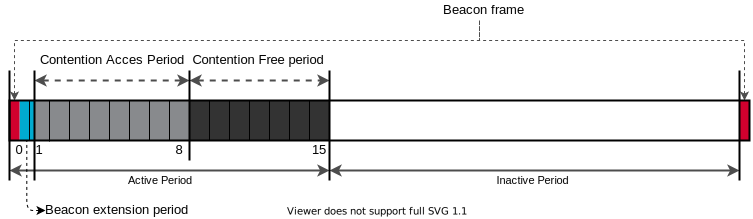
\includegraphics[scale=0.8]{images/superframe.png}
    }
    \caption{802.15.4 structure de la Superframe.}
    \label{fig:etat_art-802.15.4.superframe}
  \end{figure}

\subsubsection*{Accès au canal durant la contention acces period (CAP)}
  Durant cette période, l'accès au canal se fait par l'algotihme slotted CSMA-CA
  (Carrier Sense Multiple Access with Collision Avoidance). La figure~\ref{fig:etat_art-csmaca}
  illustre son fonctionnement.

  Les time slots de la CAP sont divisés en plus petits time slots appelés \textbf{backoff periods}.
  Un noeud du réseau maintient les variables suivantes:
  \begin{itemize}[label=\textbullet]
    \item $NB$ compte le nombre de backoff. Initialisée à 0
    \item $CW$ indique la taille de la fenêtre de congestion. Initialisée à 2
    \item $BE$ est l'exposant du backoff. Initialisée à macMinBE
  \end{itemize}

  Les variables macMinBE, macMaxBe et MCB (macCSMABackoffs) sont des constantes du protocole.
  Lorsque des paquets doivent être transmis, les variables sont d'abord initialisées.
  Ensuite, le noeud attend le prochain backoff et choisis aléatoirement un nombre entier
  $r r \in [0, 2^{BE}-1]$. Après avoir avoir attendu r backoff periods, le noeud vérifie
  si le canal est occupé en réalisant un CCA (Clear Channel Assessment).
  Si c'est le cas, $CW$ va être décrémenté et un nouveau CCA va être réalisé.
  Les paquets ne pourront être transmis qu'après trois CCA consécutifs indiquant un canal libre (i.e. $CW = 0$).
  Si le canal est occupé, $NB$ et $BE$ sont incrémentés et $CW$ est réinitialisé à 2.
  Enfin, si $NB$ n'exède pas \textit{macCSMABackoffs}, le noeud va reprendre à l'étape où un
  $r$ est choisis aléatoirement. Sinon, la communication ne sera pas établie et les paquets
  ne seront pas transférés.


\begin{figure}[H]
\begin{tikzpicture}[node distance=1.7cm]

  \node (start) [process] {\begin{tabular}{c} $NB = 0$; $CW = 2$ \\ BE = macMinBE \end{tabular}};
  \node (in1) [process, below of=start] {\begin{tabular}{c} wait until next backoff\\ period boundary\end{tabular}};
  \node (pro1) [process, below of=in1] {\begin{tabular}{c} Skip $r \in [0, 2^{BE}-1]$ \\ backoff periods \end{tabular}};
  \node (pro2) [process, below of=pro1] {Perform CCA};
  \node (dec1) [decision, below of=pro2, yshift=-0.8cm] {Channel idle?};

  \node (pro2a) [process, below of=dec1, yshift=-1cm] {\begin{tabular}{c} $NB = NB+1;CW = 2$ \\ $BE = min(BE+1, macMaxBE)$ \end{tabular}};
  \node (pro2b) [process, right of=pro2a, xshift=4cm] {$CW = CW-1$};
  \node (dec2) [decision, below of=pro2a, yshift=-1cm] {NB > MCB ?};
  \node (dec3) [decision, below of=pro2b, yshift=-1cm] {CW = 0\ ?};
  \node (fail) [endfail, below of=dec2, yshift=-1cm] {Failure};
  \node (success) [endsuccess, below of=dec3, yshift=-1cm] {Success};
  
  \draw [arrow] (start) -- (in1);
  \draw [arrow] (in1) -- (pro1);
  \draw [arrow] (pro1) -- (pro2);
  \draw [arrow] (pro2) -- (dec1);
  \draw [arrow] (dec1) -| node[anchor=south] {Yes} (pro2b);
  \draw [arrow] (dec1) -- node[anchor=east] {No} (pro2a);
  \draw [arrow] (pro2a) -- (dec2);
  \draw [arrow] (pro2b) -- (dec3);
  \draw [arrow] (dec2) -- node[anchor=east] {Yes} (fail);
  \draw [arrow] (dec2) -- node[anchor=south] {No} ++(-4,0) |- (pro1);
  \draw [arrow] (dec3) -- node[anchor=south] {No} ++(3,0) |- (pro2);
  \draw [arrow] (dec3) -- node[anchor=east] {Yes} (success);
  \end{tikzpicture}
  \caption{Schéma de l'algorithme slotted CSMA-CA.}
  \label{fig:etat_art-csmaca}
\end{figure}



\subsubsection{Accès au canal durant la contention free period} (CFP)
TODO

\subsection{Non-Beacon Enabled mode}\label{subsec:etat_art-802.15.4.nbe}

\subsection{Adressage}\label{subsec:etat_art-802.15.4.adress}

\subsection{Mécanisme d'Ack optionnel}\label{subsec:etat_art-802.15.4.ack}

%%%%%%%%%%%%%%%%%%%%% glossaries %%%%%%%%%%%%%%%%%%%%%
%\printglossaries

%%%%%%%%%%%%%%%%%%%%% bibliography %%%%%%%%%%%%%%%%%%%%%
\bibliography{res/bibliography/main,res/bibliography/rfc}
\bibliographystyle{unsrt}

%%%%%%%%%%%%%%%%%%%%% notes %%%%%%%%%%%%%%%%%%%%%
%<type>:<chapter_label_name>-<label>
%types:
% - chap: chapter
% - sec: section
% - subsec: sub section
% - fig: pictures
% - tb: tables
% - ft: foot notes
% - eq: equation
%
% chapters:
% - intro
% - state
%

\end{document}
